\documentclass[11pt, a4paper]{article}\usepackage[]{graphicx}\usepackage[]{xcolor}
% maxwidth is the original width if it is less than linewidth
% otherwise use linewidth (to make sure the graphics do not exceed the margin)
\makeatletter
\def\maxwidth{ %
  \ifdim\Gin@nat@width>\linewidth
    \linewidth
  \else
    \Gin@nat@width
  \fi
}
\makeatother

\definecolor{fgcolor}{rgb}{0.345, 0.345, 0.345}
\newcommand{\hlnum}[1]{\textcolor[rgb]{0.686,0.059,0.569}{#1}}%
\newcommand{\hlsng}[1]{\textcolor[rgb]{0.192,0.494,0.8}{#1}}%
\newcommand{\hlcom}[1]{\textcolor[rgb]{0.678,0.584,0.686}{\textit{#1}}}%
\newcommand{\hlopt}[1]{\textcolor[rgb]{0,0,0}{#1}}%
\newcommand{\hldef}[1]{\textcolor[rgb]{0.345,0.345,0.345}{#1}}%
\newcommand{\hlkwa}[1]{\textcolor[rgb]{0.161,0.373,0.58}{\textbf{#1}}}%
\newcommand{\hlkwb}[1]{\textcolor[rgb]{0.69,0.353,0.396}{#1}}%
\newcommand{\hlkwc}[1]{\textcolor[rgb]{0.333,0.667,0.333}{#1}}%
\newcommand{\hlkwd}[1]{\textcolor[rgb]{0.737,0.353,0.396}{\textbf{#1}}}%
\let\hlipl\hlkwb

\usepackage{framed}
\makeatletter
\newenvironment{kframe}{%
 \def\at@end@of@kframe{}%
 \ifinner\ifhmode%
  \def\at@end@of@kframe{\end{minipage}}%
  \begin{minipage}{\columnwidth}%
 \fi\fi%
 \def\FrameCommand##1{\hskip\@totalleftmargin \hskip-\fboxsep
 \colorbox{shadecolor}{##1}\hskip-\fboxsep
     % There is no \\@totalrightmargin, so:
     \hskip-\linewidth \hskip-\@totalleftmargin \hskip\columnwidth}%
 \MakeFramed {\advance\hsize-\width
   \@totalleftmargin\z@ \linewidth\hsize
   \@setminipage}}%
 {\par\unskip\endMakeFramed%
 \at@end@of@kframe}
\makeatother

\definecolor{shadecolor}{rgb}{.97, .97, .97}
\definecolor{messagecolor}{rgb}{0, 0, 0}
\definecolor{warningcolor}{rgb}{1, 0, 1}
\definecolor{errorcolor}{rgb}{1, 0, 0}
\newenvironment{knitrout}{}{} % an empty environment to be redefined in TeX

\usepackage{alltt}

\usepackage[top = 0.75 in, bottom = 0.75 in, left = 1 in, right = 1 in ]{geometry}

\usepackage{amsmath, amssymb, amsfonts}
\usepackage{enumerate}
\usepackage{array}
\usepackage{multirow}
\usepackage{dingbat}
\usepackage{fontawesome5}
\usepackage{tasks}
\usepackage{bbding}
\usepackage{twemojis}
% how to use bull's eye ----- \scalebox{2.0}{\twemoji{bullseye}}
\usepackage{fontspec}
\usepackage{customdice}
% how to put dice face ------ \dice{2}

\title{MSMS 106 : Practical 12}
\author{Ananda Biswas}
\date{\today}

\newfontface\ifr{IndieFlower-Regular.ttf}
% how to use ---- {\ifr write text here}
\IfFileExists{upquote.sty}{\usepackage{upquote}}{}
\begin{document}

\maketitle


\section*{\faArrowAltCircleRight[regular] \textcolor{blue}{Objective}}

\hspace{1cm} To simulate and calculate total sales for 4 regions over 5 months and plot the results.




\section*{\faArrowAltCircleRight[regular] \textcolor{blue}{R Program, Plot and Interpretation}}

\leftpointright \hspace{0.2cm} Data simulation
\begin{knitrout}
\definecolor{shadecolor}{rgb}{0.969, 0.969, 0.969}\color{fgcolor}\begin{kframe}
\begin{alltt}
\hldef{sales} \hlkwb{<-} \hlkwd{c}\hldef{()}
\hldef{temp} \hlkwb{<-} \hlkwd{c}\hldef{(}\hlnum{2}\hldef{,} \hlnum{4}\hldef{,} \hlnum{7}\hldef{,} \hlnum{10}\hldef{,} \hlnum{5}\hldef{)}

\hlkwa{for} \hldef{(i} \hlkwa{in} \hlnum{1}\hlopt{:}\hlnum{4}\hldef{) \{}
  \hlkwa{for} \hldef{(j} \hlkwa{in} \hlnum{1}\hlopt{:}\hlnum{5}\hldef{) \{}
    \hldef{sales} \hlkwb{<-} \hlkwd{append}\hldef{(sales,} \hlkwd{round}\hldef{(}\hlkwd{rnorm}\hldef{(}\hlnum{1}\hldef{,} \hlnum{10}\hlopt{*}\hldef{i} \hlopt{+} \hlnum{20}\hlopt{*}\hldef{temp[j],} \hlnum{1}\hldef{),} \hlkwc{digits} \hldef{=} \hlnum{2}\hldef{))}
  \hldef{\}}
\hldef{\}}

\hldef{regions} \hlkwb{<-} \hlkwd{rep}\hldef{(}\hlkwd{c}\hldef{(}\hlsng{"Region1"}\hldef{,} \hlsng{"Region2"}\hldef{,} \hlsng{"Region3"}\hldef{,} \hlsng{"Region4"}\hldef{),} \hlkwd{rep}\hldef{(}\hlnum{5}\hldef{,} \hlnum{4}\hldef{))}
\hldef{months} \hlkwb{<-} \hlkwd{rep}\hldef{(}\hlkwd{c}\hldef{(}\hlsng{"Month1"}\hldef{,} \hlsng{"Month2"}\hldef{,} \hlsng{"Month3"}\hldef{,} \hlsng{"Month4"}\hldef{,} \hlsng{"Month5"}\hldef{),} \hlnum{4}\hldef{)}

\hldef{sales_df} \hlkwb{<-} \hlkwd{data.frame}\hldef{(}\hlkwc{region} \hldef{=} \hlkwd{as.factor}\hldef{(regions),}
                       \hlkwc{month} \hldef{=} \hlkwd{as.factor}\hldef{(months),}
                       \hlkwc{sales} \hldef{= sales)}

\hlcom{# View(sales_df)}
\end{alltt}
\end{kframe}
\end{knitrout}


\begin{knitrout}
\definecolor{shadecolor}{rgb}{0.969, 0.969, 0.969}\color{fgcolor}\begin{kframe}
\begin{alltt}
\hlkwd{summary}\hldef{(sales_df)}
\end{alltt}
\begin{verbatim}
##      region     month       sales       
##  Region1:5   Month1:4   Min.   : 50.24  
##  Region2:5   Month2:4   1st Qu.: 98.53  
##  Region3:5   Month3:4   Median :124.96  
##  Region4:5   Month4:4   Mean   :137.09  
##              Month5:4   3rd Qu.:172.28  
##                         Max.   :239.35
\end{verbatim}
\end{kframe}
\end{knitrout}

\begin{knitrout}
\definecolor{shadecolor}{rgb}{0.969, 0.969, 0.969}\color{fgcolor}\begin{kframe}
\begin{alltt}
\hlkwd{library}\hldef{(tidyverse)}
\end{alltt}
\end{kframe}
\end{knitrout}

\newpage

\leftpointright \hspace{0.2cm} Region-wise sales
\begin{knitrout}
\definecolor{shadecolor}{rgb}{0.969, 0.969, 0.969}\color{fgcolor}\begin{kframe}
\begin{alltt}
\hldef{region_sale} \hlkwb{<-} \hldef{sales_df} \hlopt
  \hlkwd{group_by}\hldef{(region)} \hlopt
  \hlkwd{summarise}\hldef{(}\hlkwc{total_sale} \hldef{=} \hlkwd{sum}\hldef{(sales))}
\end{alltt}
\end{kframe}
\end{knitrout}

\begin{knitrout}
\definecolor{shadecolor}{rgb}{0.969, 0.969, 0.969}\color{fgcolor}\begin{kframe}
\begin{alltt}
\hldef{region_sale} \hlopt
  \hlkwd{ggplot}\hldef{(}\hlkwd{aes}\hldef{(}\hlkwc{x} \hldef{= region,} \hlkwc{y} \hldef{= total_sale))} \hlopt{+}
  \hlkwd{geom_col}\hldef{(}\hlkwc{fill} \hldef{=} \hlkwd{c}\hldef{(}\hlsng{"#e1d216"}\hldef{,} \hlsng{"#16d5e1"}\hldef{,} \hlsng{"#9416e1"}\hldef{,} \hlsng{"#f81a7f"}\hldef{),}
           \hlkwc{col} \hldef{=} \hlsng{"black"}\hldef{)} \hlopt{+}
  \hlkwd{geom_text}\hldef{(}\hlkwd{aes}\hldef{(}\hlkwc{label} \hldef{= total_sale),}
            \hlkwc{vjust} \hldef{=} \hlopt{-}\hlnum{0.5}\hldef{,}
            \hlkwc{size} \hldef{=} \hlnum{4}\hldef{)} \hlopt{+}
  \hlkwd{labs}\hldef{(}\hlkwc{x} \hldef{=} \hlsng{"Region"}\hldef{,} \hlkwc{y} \hldef{=} \hlsng{"Total Sale"}\hldef{,}
       \hlkwc{title} \hldef{=} \hlsng{"Sales in Different Regions"}\hldef{)}
\end{alltt}
\end{kframe}
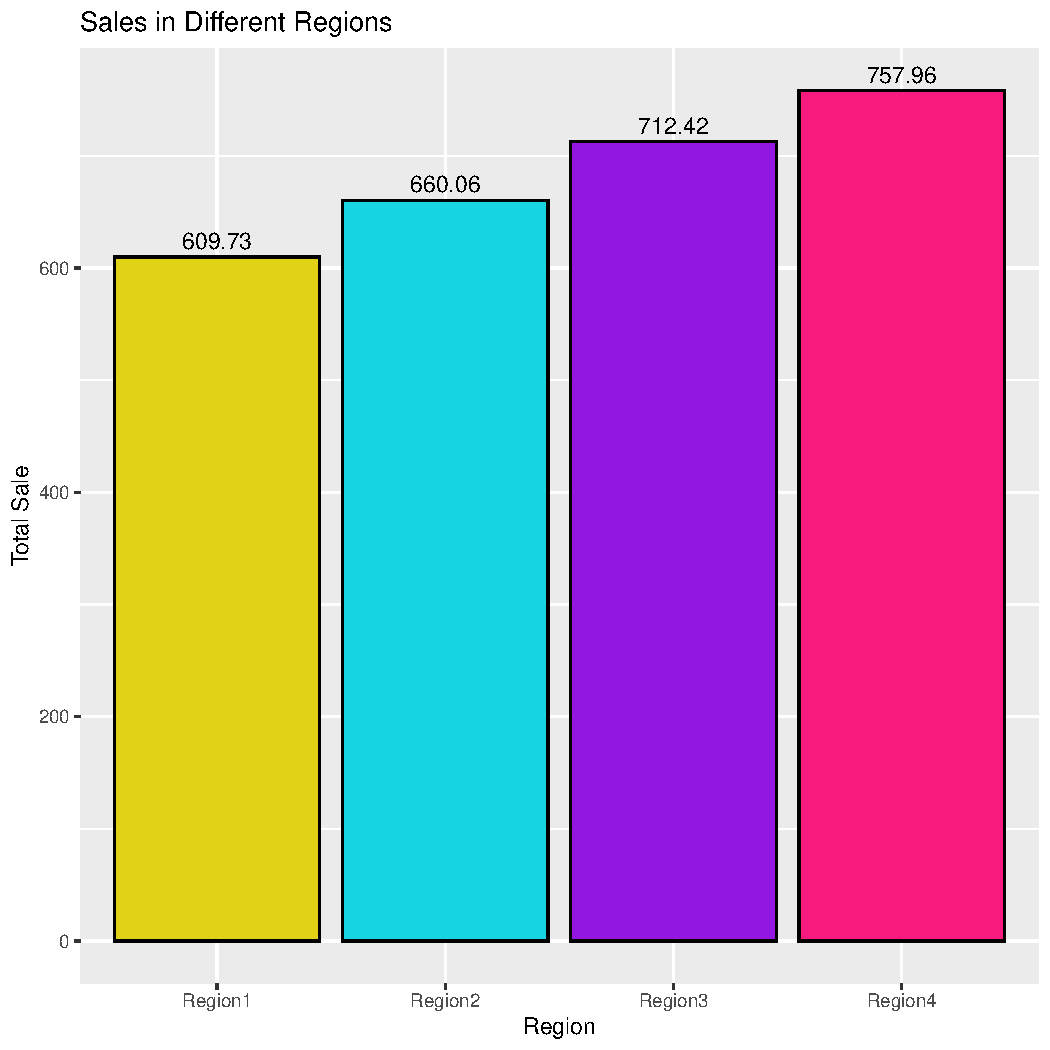
\includegraphics[width=\maxwidth]{figure/unnamed-chunk-5-1} 
\end{knitrout}

\smallpencil {\ifr When total sale of all 5 months is considered, Region1 has the lowest sales and Region4 has the highest sales.} \\


\newpage

\leftpointright \hspace{0.2cm} Month-wise sales

\begin{knitrout}
\definecolor{shadecolor}{rgb}{0.969, 0.969, 0.969}\color{fgcolor}\begin{kframe}
\begin{alltt}
\hldef{month_sales} \hlkwb{<-} \hldef{sales_df} \hlopt
  \hlkwd{group_by}\hldef{(month)} \hlopt
  \hlkwd{summarise}\hldef{(}\hlkwc{total_sale} \hldef{=} \hlkwd{sum}\hldef{(sales))}
\end{alltt}
\end{kframe}
\end{knitrout}


\begin{knitrout}
\definecolor{shadecolor}{rgb}{0.969, 0.969, 0.969}\color{fgcolor}\begin{kframe}
\begin{alltt}
\hldef{month_sales} \hlopt
  \hlkwd{ggplot}\hldef{(}\hlkwd{aes}\hldef{(}\hlkwc{x} \hldef{= month,} \hlkwc{y} \hldef{= total_sale))} \hlopt{+}
  \hlkwd{geom_col}\hldef{(}\hlkwc{fill} \hldef{=} \hlkwd{c}\hldef{(}\hlsng{"#59f814"}\hldef{,} \hlsng{"#54e614"}\hldef{,} \hlsng{"#4fd514"}\hldef{,} \hlsng{"#46ba14"}\hldef{,} \hlsng{"#41ac12"}\hldef{),}
           \hlkwc{col} \hldef{=} \hlsng{"black"}\hldef{)} \hlopt{+}
  \hlkwd{geom_text}\hldef{(}\hlkwd{aes}\hldef{(}\hlkwc{label} \hldef{= total_sale),}
            \hlkwc{vjust} \hldef{=} \hlopt{-}\hlnum{0.5}\hldef{,}
            \hlkwc{size} \hldef{=} \hlnum{4}\hldef{)} \hlopt{+}
  \hlkwd{labs}\hldef{(}\hlkwc{x} \hldef{=} \hlsng{"Month"}\hldef{,} \hlkwc{y} \hldef{=} \hlsng{"Total Sale"}\hldef{,}
       \hlkwc{title} \hldef{=} \hlsng{"Month-wise Total Sales"}\hldef{)}
\end{alltt}
\end{kframe}
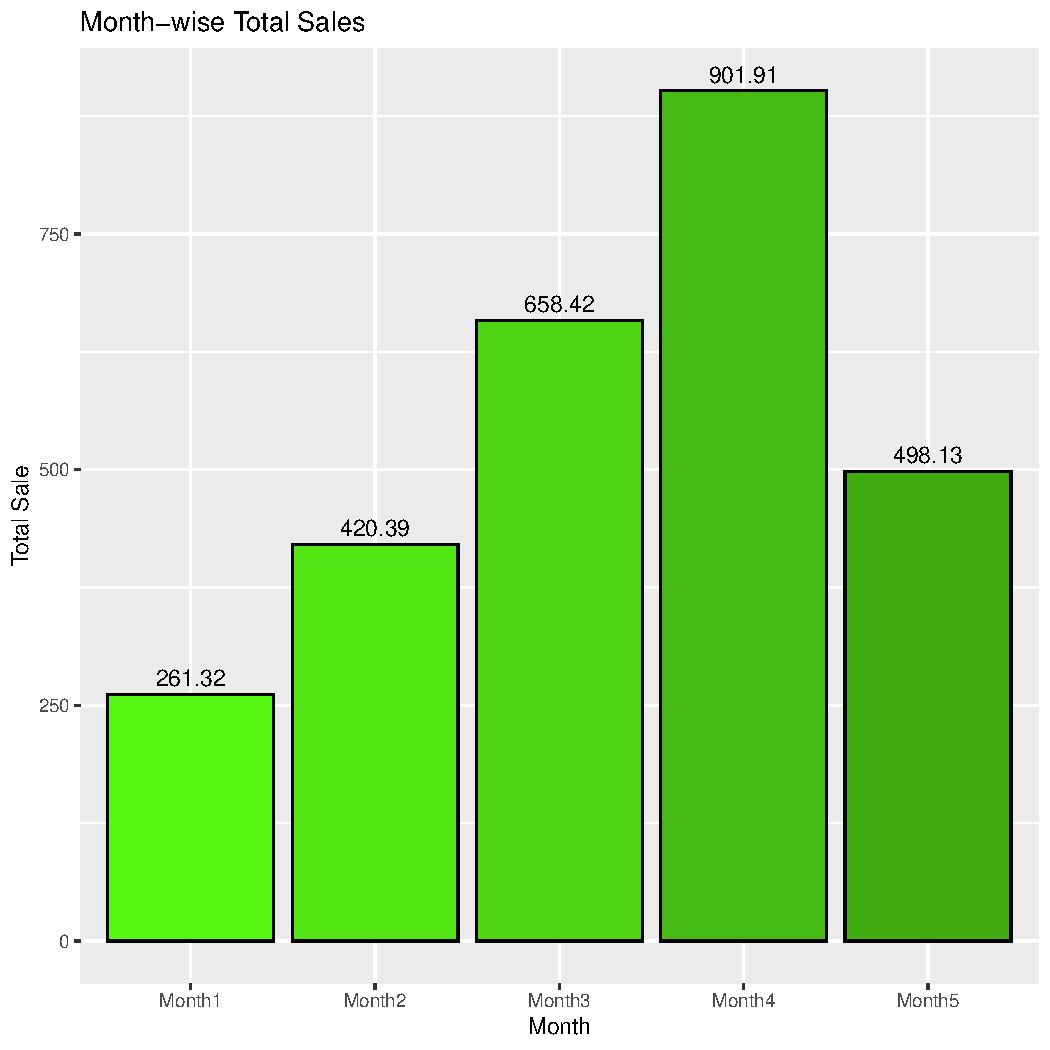
\includegraphics[width=\maxwidth]{figure/unnamed-chunk-7-1} 
\end{knitrout}

\smallpencil {\ifr When we aggregate sales of all the regions over different months, we see that there is a sharp increase in total sales over months.}



\section*{\faArrowAltCircleRight[regular] \textcolor{blue}{Conclusion}}

\smallpencil \hspace{1cm} {\ifr Our data have an increasing trend of total sales over months. Also, "Region4" has highest number of sales.}

\end{document}
